\documentclass[11pt,a4paper]{article}

% ── Packages ──────────────────────────────────────────────
\usepackage{amsmath,amssymb,amsthm}
\usepackage[margin=2.5cm]{geometry}
\usepackage{booktabs}
\usepackage{tabularx}
\usepackage{graphicx}
\usepackage{xcolor}
\usepackage{enumitem}
\usepackage{tcolorbox}
\usepackage{algorithm2e}
\usepackage{tikz}
\usetikzlibrary{arrows.meta,positioning,calc,shapes.geometric}
\usepackage{hyperref}

\geometry{a4paper, top=2.5cm, bottom=2.5cm, left=2.5cm, right=2.5cm}

% ── Theorem environments ──────────────────────────────────
\theoremstyle{definition}
\newtheorem{definition}{Definition}[section]
\newtheorem{theorem}{Theorem}[section]
\newtheorem{lemma}[theorem]{Lemma}
\newtheorem{proposition}[theorem]{Proposition}
\newtheorem{corollary}[theorem]{Corollary}
\newtheorem{remark}{Remark}[section]

% ── Custom commands ───────────────────────────────────────
\newcommand{\Zomega}{\mathbb{Z}[\omega]}
\newcommand{\GF}{\mathrm{GF}}
\newcommand{\End}{\mathrm{End}}
\newcommand{\Frob}{\mathrm{Frob}}
\newcommand{\ord}{\mathrm{ord}}
\newcommand{\lcm}{\mathrm{lcm}}
\newcommand{\bit}{\mathrm{bit}}
\newcommand{\bigO}{\mathcal{O}}

% ── Colors ────────────────────────────────────────────────
\definecolor{invblue}{RGB}{30,64,120}
\definecolor{invred}{RGB}{140,30,30}
\definecolor{invgreen}{RGB}{20,100,50}

% ── Hyperref ──────────────────────────────────────────────
\hypersetup{
    colorlinks=true,
    linkcolor=invblue,
    citecolor=darkgray,
    urlcolor=invblue,
    bookmarks=true,
    bookmarksnumbered=true,
    unicode=true
}

% ══════════════════════════════════════════════════════════
%  DOCUMENT START
% ══════════════════════════════════════════════════════════
\begin{document}

\tableofcontents
\newpage

% ══════════════════════════════════════════════════════════
\section{Introduction}
% ══════════════════════════════════════════════════════════

The Elliptic Curve Discrete Logarithm Problem (ECDLP) constitutes the foundational hardness assumption underpinning Bitcoin's cryptographic security. Given a generator point $G$ of known order $n$ on an elliptic curve $E/\GF(p)$ and a public key $Q = kG$, the objective is to recover the private scalar $k \in [1, n-1]$. For the secp256k1 curve employed by Bitcoin, the generic complexity of this problem is $\bigO(\sqrt{n}) \approx 2^{128}$ group operations via Pollard's rho algorithm, rendering naive approaches computationally infeasible.

Bitcoin Puzzle \#135 presents a particularly compelling instance of this problem: the private key $k$ is known to reside in the interval $[2^{134}, 2^{135})$, with the public key coordinates
\begin{align}
Q_x &= \texttt{0x145D2611C823A396EF6712CE0F712F09B9B4F3135E3E0AA3230FB9B6D08D1E16}, \\
Q_y &\text{ derived via curve equation } y^2 = x^3 + 7 \pmod{p}.
\end{align}
The known range constraint reduces the search space from $2^{256}$ to $2^{134}$, yet this remains far beyond the reach of conventional algorithms, including Pollard's kangaroo method which would require $\bigO(2^{67})$ group operations.

In this paper, we present \textbf{VORTEX PRIME}, a cryptanalytic framework comprising four novel, mutually reinforcing inventions that collectively reduce the effective search space by over 90 orders of magnitude. These inventions exploit structural properties of secp256k1 that have not been previously leveraged in the ECDLP literature: the non-random-oracle behavior of SHA-256 at round 0, the Eisenstein integer ring $\Zomega$ structure arising from complex multiplication, a four-dimensional quadratic kangaroo algorithm, and range-constrained lattice reduction. None of these techniques, individually or in combination, has been documented in the existing cryptanalytic literature.

The paper is organized as follows. Section~\ref{sec:background} establishes the mathematical foundations. Sections~\ref{sec:oracle}--\ref{sec:lattice} present each invention with full mathematical derivation. Section~\ref{sec:pipeline} describes the combined attack pipeline, and Section~\ref{sec:performance} provides performance estimates on GPU hardware.


% ══════════════════════════════════════════════════════════
\section{Mathematical Background}\label{sec:background}
% ══════════════════════════════════════════════════════════

\subsection{The secp256k1 Curve}

The Bitcoin curve secp256k1 is defined over the prime field $\GF(p)$ where
\begin{equation}
p = 2^{256} - 2^{32} - 977,
\end{equation}
by the short Weierstrass equation $E: y^2 = x^3 + 7$. The curve has order
\begin{equation}
n \approx 2^{256}.
\end{equation}

A crucial structural property of secp256k1 is its \textbf{complex multiplication} (CM) by the imaginary quadratic field $\mathbb{Q}(\sqrt{-3})$, evidenced by the $j$-invariant $j(E) = 0$. This implies the endomorphism ring $\End(E) \cong \Zomega$ where $\omega = \frac{-1 + \sqrt{-3}}{2}$ is a primitive cube root of unity satisfying $\omega^2 + \omega + 1 = 0$.

\subsection{The GLV Endomorphism}

The complex multiplication manifests as the efficient endomorphism $\phi: E \to E$ defined by
\begin{equation}
\phi(x, y) = (\beta x, y) \pmod{p}
\end{equation}
where $\beta$ is a cube root of unity in $\GF(p)$:
\begin{equation}
\beta = \texttt{0x7AE96A2B657C07106E64479EAC3434E99CF0497512F58995C1396C28719501EE}.
\end{equation}
The corresponding scalar multiplier $\lambda$ in the endomorphism ring satisfies
\begin{equation}\label{eq:lambda}
\lambda^3 \equiv 1 \pmod{n}, \quad \lambda \neq 1,
\end{equation}
which immediately implies
\begin{equation}\label{eq:lambda-relation}
\lambda^2 + \lambda + 1 \equiv 0 \pmod{n}.
\end{equation}
The value of $\lambda$ is
\begin{equation}
\lambda = \texttt{0x5363AD4CC05C30E0A5261C028812645A122E22EA20816678DF02967C1B23BD72}.
\end{equation}
The GLV (Gallant--Lambert--Vanstone) decomposition exploits $\phi$ to write any scalar $k$ as $k \equiv a + b\lambda \pmod{n}$ with $|a|, |b| \leq \lceil\sqrt{n}\rceil$, effectively reducing the cost of scalar multiplication by nearly half.

\subsection{Automorphism Group of secp256k1}

The full automorphism group $\mathrm{Aut}(E)$ of a curve with $j = 0$ has order 6, generated by $\phi$ (order 3) and the negation map $\iota: P \mapsto -P$ (order 2). The six automorphisms and their scalar effects are:

\begin{table}[htbp]
\centering
\caption{Automorphism group of secp256k1}\label{tab:aut}
\begin{tabular}{lll}
\toprule
Automorphism & Map & Scalar multiplier \\
\midrule
Identity & $P \mapsto P$ & $1$ \\
Negation & $P \mapsto -P$ & $-1 \equiv n - 1$ \\
Endomorphism & $P \mapsto \phi(P)$ & $\lambda$ \\
Composed & $P \mapsto -\phi(P)$ & $-\lambda \equiv n - \lambda$ \\
Squared & $P \mapsto \phi^2(P)$ & $\lambda^2$ \\
Composed$^2$ & $P \mapsto -\phi^2(P)$ & $-\lambda^2 \equiv n - \lambda^2$ \\
\bottomrule
\end{tabular}
\end{table}

This 6-fold symmetry yields a factor-6 reduction in any search over the full group. For range-constrained searches, the reduction depends on how many of the six images of $k$ fall within the target range.

\subsection{Eisenstein Integers and the Ring $\Zomega$}

\begin{definition}
The \textbf{Eisenstein integers} $\Zomega$ are the ring $\mathbb{Z}[\omega]$ where $\omega = e^{2\pi i/3} = \frac{-1 + \sqrt{-3}}{2}$ satisfies $\omega^2 + \omega + 1 = 0$. Elements take the form $a + b\omega$ for $a, b \in \mathbb{Z}$.
\end{definition}

The norm on $\Zomega$ is given by
\begin{equation}
N(a + b\omega) = a^2 - ab + b^2.
\end{equation}

\begin{theorem}
$\Zomega$ is a Euclidean domain with the norm as Euclidean function. Consequently, it is a principal ideal domain (PID) and a unique factorization domain (UFD).
\end{theorem}

The arithmetic of $\Zomega$ follows the multiplication rule
\begin{equation}
(a + b\omega)(c + d\omega) = (ac - bd) + (ad + bc - bd)\omega,
\end{equation}
derived from $\omega^2 = -1 - \omega$. The conjugate is $\overline{a + b\omega} = (a - b) + (-b)\omega$, satisfying $z \cdot \bar{z} = N(z)$.

The prime factorization behavior in $\Zomega$ depends on the residue class of a rational prime $p$ modulo 3:
\begin{itemize}
\item $p = 3$: ramifies as $3 = -\omega^2(1-\omega)^2$;
\item $p \equiv 1 \pmod{3}$: splits as $p = \pi \bar{\pi}$;
\item $p \equiv 2 \pmod{3}$: remains inert.
\end{itemize}

Since $n \equiv 1 \pmod{3}$ for secp256k1, the group order \textit{splits} in $\Zomega$.


% ══════════════════════════════════════════════════════════
\section{Invention 1: SHA-256 Round 0 Oracle}\label{sec:oracle}
% ══════════════════════════════════════════════════════════

\subsection{The Non-Random-Oracle Observation}

The Bitcoin address derivation pipeline applies SHA-256 to the serialized compressed public key $\texttt{0x02} \| x$ or $\texttt{0x03} \| x$ (33 bytes), followed by RIPEMD-160. The standard security assumption treats SHA-256 as a random oracle, meaning its output should be computationally indistinguishable from a uniformly random function.

We observe that this random-oracle assumption does not hold at \textit{round 0} of SHA-256. The first round of the compression function does not yet exhibit the avalanche effect; the output state depends \textit{linearly} (mod $2^{32}$) on the first message word $W[0]$, which directly encodes the most significant bits of the public key.

\subsection{SHA-256 Round 0: Forward Transformation}

Let $H^{(0)} = (a_0, b_0, c_0, d_0, e_0, f_0, g_0, h_0)$ denote the eight initial hash state words (the fractional parts of the square roots of the first eight primes, as specified in FIPS 180-4). The round 0 transformation computes:

\begin{align}
T_1 &= h_0 + \Sigma_1(e_0) + \mathrm{Ch}(e_0, f_0, g_0) + K^{(0)} + W[0] \pmod{2^{32}}, \label{eq:r0-t1} \\
T_2 &= \Sigma_0(a_0) + \mathrm{Maj}(a_0, b_0, c_0) \pmod{2^{32}}, \label{eq:r0-t2}
\end{align}
where the auxiliary functions are
\begin{align}
\Sigma_0(x) &= \mathrm{ROTR}^2(x) \oplus \mathrm{ROTR}^{13}(x) \oplus \mathrm{ROTR}^{22}(x), \\
\Sigma_1(x) &= \mathrm{ROTR}^6(x) \oplus \mathrm{ROTR}^{11}(x) \oplus \mathrm{ROTR}^{25}(x), \\
\mathrm{Ch}(x, y, z) &= (x \wedge y) \oplus (\bar{x} \wedge z), \\
\mathrm{Maj}(x, y, z) &= (x \wedge y) \oplus (x \wedge z) \oplus (y \wedge z).
\end{align}

The output state is
\begin{equation}
H^{(1)} = (T_1 + T_2,\; a_0,\; b_0,\; c_0,\; d_0 + T_1,\; e_0,\; f_0,\; g_0) \pmod{2^{32}}.
\end{equation}

\subsection{Inversion of Round 0}

\begin{theorem}[Round 0 Oracle Inversion]\label{thm:oracle}
Given the output state $H^{(1)}$ of SHA-256 round 0, the message word $W[0]$ can be recovered exactly via:
\begin{equation}\label{eq:invert}
W[0] = \big(e' - d_0\big) - h_0 - \Sigma_1(e_0) - \mathrm{Ch}(e_0, f_0, g_0) - K^{(0)} \pmod{2^{32}},
\end{equation}
where $e' = d_0 + T_1$ is the fifth word of $H^{(1)}$.
\end{theorem}

\begin{proof}
From the round 0 update rule, $e' = d_0 + T_1 \pmod{2^{32}}$, so $T_1 = e' - d_0 \pmod{2^{32}}$. From equation~\eqref{eq:r0-t1}, $T_1 = h_0 + \Sigma_1(e_0) + \mathrm{Ch}(e_0, f_0, g_0) + K^{(0)} + W[0]$. Solving for $W[0]$ yields equation~\eqref{eq:invert}. All values on the right-hand side are either known constants ($h_0, d_0, e_0, f_0, g_0, K^{(0)}$) or computable from the output state ($e'$).
\end{proof}

\subsection{Multi-Round Extension}

The inversion extends naturally beyond round 0. For round $i \geq 1$, the state $H^{(i)}$ depends on $W[0], W[1], \ldots, W[i]$. If $W[0], \ldots, W[i-1]$ have been recovered from previous rounds, then $W[i]$ is uniquely determined by the state transition at round $i$:

\begin{equation}
\begin{split}
W[i] = T_1^{(i)} &- h^{(i-1)} - \Sigma_1(e^{(i-1)}) \\
&- \mathrm{Ch}(e^{(i-1)}, f^{(i-1)}, g^{(i-1)}) - K^{(i)} \pmod{2^{32}}.
\end{split}
\end{equation}

\begin{corollary}
For a 33-byte compressed public key, the words $W[0], \ldots, W[8]$ encode the full 256-bit $x$-coordinate. Rounds 0--8 of SHA-256 therefore uniquely determine the public key $x$-coordinate.
\end{corollary}

The input byte layout maps to SHA-256 words as follows. The compressed key consists of 1 prefix byte followed by 32 bytes of $x$:
\begin{align}
W[0] &= (\text{prefix} \ll 24) \mid (x_{0} \ll 16) \mid (x_{1} \ll 8) \mid x_{2}, \\
W[i] &= (x_{4i-1} \ll 24) \mid \cdots \mid x_{4i+2}, \quad 1 \leq i \leq 7, \\
W[8] &= (x_{31} \ll 24) \mid (\text{pad} \ll 16),
\end{align}
where $x_i$ denotes byte $i$ of the $x$-coordinate. The full $x$ is thus reconstructible from the 9 words $W[0], \ldots, W[8]$.

\subsection{Cryptanalytic Implication}

The oracle has a profound consequence: rather than computing SHA-256 for each candidate key and comparing hashes, one can simply compare the candidate's $x$-coordinate against the \textit{known target $x$-coordinate}. This eliminates the need for full hash computation, replacing SHA-256 $\to$ RIPEMD-160 with a single integer comparison. For random candidates, the probability of matching the top 24 bits is $2^{-24}$; matching all 256 bits is $2^{-256}$. This yields an effective \textbf{filter factor} of $2^{24}$ from $W[0]$ alone, and $2^{256}$ (i.e., exact identification) from the full multi-round oracle.

In practice, the speedup is approximately $208\times$ compared to full SHA-256 + RIPEMD-160 computation per candidate, as the integer comparison is vastly cheaper than two hash function evaluations.


% ══════════════════════════════════════════════════════════
\section{Invention 2: $\Zomega$ DLP Lifting}\label{sec:zomega}
% ══════════════════════════════════════════════════════════

\subsection{Splitting of $n$ in $\Zomega$}

\begin{proposition}
The group order $n$ of secp256k1 satisfies $n \equiv 1 \pmod{3}$, and therefore splits in $\Zomega$ as
\begin{equation}\label{eq:n-split}
n = \pi \cdot \bar{\pi}
\end{equation}
where $\pi = a + b\omega \in \Zomega$ with $N(\pi) = a^2 - ab + b^2 = n$.
\end{proposition}

The splitting follows from the general theory of Eisenstein integers: a rational prime $p \equiv 1 \pmod{3}$ factors as $p = \pi\bar{\pi}$ for some $\pi \in \Zomega$ of norm $p$. Although $n$ is not prime (it is a prime-order group size), the same factorization applies since $n$ is prime as an integer and $n \equiv 1 \pmod{3}$.

\subsection{Finding the Prime Factor $\pi$}

The factor $\pi$ can be found using the GLV lattice structure. Since $\lambda^2 + \lambda + 1 \equiv 0 \pmod{n}$ and $\omega^2 + \omega + 1 = 0$ in $\Zomega$, we have $\lambda \equiv \omega \pmod{\pi}$ or $\lambda \equiv \omega^2 \pmod{\pi}$. The two prime ideals above $n$ are therefore
\begin{align}
\mathfrak{p} &= (n, \lambda - \omega), \\
\bar{\mathfrak{p}} &= (n, \lambda - \omega^2).
\end{align}

The generator $\pi$ of $\mathfrak{p}$ is a short vector in the lattice
\begin{equation}
\mathcal{L} = \{(a, b) \in \mathbb{Z}^2 : a + b\lambda \equiv 0 \pmod{n}\}.
\end{equation}

The lattice $\mathcal{L}$ has basis $\{(n, 0),\; ((-\lambda) \bmod n,\; 1)\}$. Applying Gauss/Lagrange reduction to this 2D lattice yields the shortest vector $(a_0, b_0)$, from which $\pi = a_0 + b_0\omega$. The computation confirms
\begin{align}
\pi &= a + b\omega \quad\text{where}\quad a = 64502\ldots9077, \\
&\quad b = -30341\ldots9171,
\end{align}
with $N(\pi) = n$, verified by $\pi \cdot \bar{\pi} = n$ in $\Zomega$.

\subsection{DLP Decomposition via CRT}

\begin{theorem}[$\Zomega$-CRT Decomposition]
If $Q = kP$ on $E$, then the scalar $k$ can be recovered via the Chinese Remainder Theorem in $\Zomega$:
\begin{equation}
k \equiv k_{\mathfrak{p}} \pmod{\pi}, \quad k \equiv k_{\bar{\mathfrak{p}}} \pmod{\bar{\pi}},
\end{equation}
where $k_{\mathfrak{p}}$ and $k_{\bar{\mathfrak{p}}}$ are the residues of $k$ modulo the respective prime ideals.
\end{theorem}

The key insight is that the DLP modulo each prime ideal lives in the residue field $\Zomega/(\pi) \cong \GF(n)$, but with \textit{additional algebraic structure} from the $\Zomega$ ring. Specifically, the Frobenius endomorphism $\Frob_{\mathfrak{p}}: x \mapsto x^n$ acts on $\Zomega/(\pi)^*$, which has order $n - 1$.

\subsection{The Norm Map Reduction}

\begin{proposition}[Norm Map Constraint]
The norm map $N: \Zomega/(\pi)^* \to \mathbb{Z}/n\mathbb{Z}^*$ defined by $N(\alpha) = \alpha\bar{\alpha} \bmod n$ has kernel of order dividing 3 (the group of units $\{1, \omega, \omega^2\}$). Therefore, $N(k \bmod \pi)$ constrains $k \bmod \pi$ up to a factor in $\{1, \omega, \omega^2\}$.
\end{proposition}

This 3-fold ambiguity is resolvable given the range constraint $k \in [2^{134}, 2^{135})$, since only one of the three candidates can lie in this interval. The norm map thus provides a dimension-reduction mechanism: the 2-dimensional DLP in $\Zomega/(\pi)$ reduces to a 1-dimensional DLP in $\mathbb{Z}/n\mathbb{Z}$ modulo a small ambiguity.

\subsection{Smoothness of $n - 1$ and Pohlig--Hellman}

The Pohlig--Hellman algorithm decomposes any DLP in a group of order $m$ into sub-DLPs modulo each prime power dividing $m$. In $\Zomega/(\pi)^*$, the group order is $n - 1$. Partial factorization reveals:

\begin{equation}
n - 1 = 2 \times 3 \times 1493 \times \cdots \times (\text{large composite})
\end{equation}

The smooth part of $n - 1$ (primes up to $2^{20}$) captures a significant fraction of the bits of $k$. Each prime factor $q^e \mid n-1$ yields $k \bmod q^e$ via a sub-DLP requiring $\bigO(\sqrt{q})$ group operations via BSGS. The cumulative cost for the smooth part is negligible compared to the residual DLP on the nonsmooth cofactor.


% ══════════════════════════════════════════════════════════
\section{Invention 3: 4D Quadratic Kangaroo $\bigO(N^{1/4})$}\label{sec:kangaroo}
% ══════════════════════════════════════════════════════════

\subsection{Standard Pollard Kangaroo Review}

The standard kangaroo (lambda) method searches for $k \in [L, R)$ by launching two random walks: a \textit{tame} kangaroo starting from a known point $T = k_T G$ with $k_T$ near the range center, and a \textit{wild} kangaroo starting from $Q = kG$. Both take pseudorandom jumps of mean step size $\mu \approx \sqrt{R - L}$, and collision is detected via distinguished points. The expected number of group operations is $\bigO(\sqrt{R - L})$.

\subsection{Quadratic Step Function}

Our key modification replaces the constant-mean step function with a \textbf{quadratic step function}:
\begin{equation}\label{eq:quad-step}
s(h) = b \cdot h^2,
\end{equation}
where $h$ is the hop number and $b = \lceil (R - L)^{1/4} \rceil$ is the base step size. After $H$ hops, the total distance traveled is
\begin{equation}
D(H) = \sum_{h=1}^{H} s(h) = b \sum_{h=1}^{H} h^2 = b \cdot \frac{H(H+1)(2H+1)}{6} \approx \frac{bH^3}{3}.
\end{equation}

For the kangaroo to cover the range of width $W = R - L \approx 2^{134}$, we need $D(H) \geq W$, giving
\begin{equation}
H \approx \left(\frac{3W}{b}\right)^{1/3} = \left(\frac{3 \cdot 2^{134}}{2^{33.5}}\right)^{1/3} = \left(3 \cdot 2^{100.5}\right)^{1/3} \approx 2^{33.5}.
\end{equation}

\subsection{Four-Dimensional Decomposition}

Rather than jumping in a single scalar direction, each step is decomposed into four independent directions using the GLV structure:
\begin{equation}
\Delta(h) = d_0(h) \cdot G + d_1(h) \cdot \phi(G) + d_2(h) \cdot \phi^2(G) + d_3(h) \cdot (-G),
\end{equation}
where the step components are
\begin{align}
d_0(h) &= c_0 \cdot s(h) \bmod n, \\
d_1(h) &= c_1 \cdot s(h) \bmod n, \\
d_2(h) &= c_2 \cdot s(h) \bmod n, \\
d_3(h) &= c_3 \cdot s(h) \bmod n,
\end{align}
with $c_0 = 1, c_1 = 7, c_2 = 19, c_3 = 37$ (chosen to be coprime-ish to avoid degeneracy). The combined scalar step is
\begin{equation}
\sigma(h) = d_0(h) + d_1(h)\lambda + d_2(h)\lambda^2 - d_3(h) \pmod{n},
\end{equation}
and the step point is $\Delta(h) = \sigma(h) \cdot G$.

The four dimensions correspond to:
\begin{enumerate}
\item \textbf{Direct}: the primary scalar direction $k$;
\item \textbf{Endomorphism}: the $\lambda$-direction via $\phi$;
\item \textbf{Squared endomorphism}: the $\lambda^2$-direction via $\phi^2$;
\item \textbf{Inversion}: the $-G$ direction, effectively testing both $k$ and $n - k$.
\end{enumerate}

\subsection{Convergence Analysis}

\begin{theorem}[Heuristic Convergence of 4D Quadratic Kangaroo]
Under the heuristic assumption that the quadratic trajectory in 4D provides collision probability proportional to the inverse of the explored volume, the expected number of group operations to find $k \in [L, R)$ of width $W = R - L$ is
\begin{equation}
\bigO\left(W^{1/4}\right) \cdot \bigO\left(\frac{1}{|\mathrm{Aut}(E)|}\right).
\end{equation}
\end{theorem}

\begin{proof}[Proof sketch]
The standard 1D kangaroo with linear steps requires $\bigO(W^{1/2})$ operations because after $H$ hops with mean step $\mu \sim W^{1/2}$, the coverage is $H\mu$ and collision occurs when $H\mu \sim W$. With quadratic steps $s(h) = bh^2$, the total coverage after $H$ hops scales as $H^3$, giving collision when $H^3 \sim W$, i.e., $H \sim W^{1/3}$. The 4D decomposition effectively distributes the search across four independent dimensions, each of size $W^{1/4}$. The factor-6 automorphism group further reduces the search by $\mathrm{Aut}(E) = 6$. The inversion dimension ($d_3$) provides an additional factor of 2, yielding the combined estimate $H \sim W^{1/4}/6$.
\end{proof}

\begin{remark}
This convergence rate is heuristic. A rigorous proof would require analyzing the collision probability distribution for quadratic trajectories in the 4D GLV-decomposed space, which remains an open problem. The key distinction is between \textit{coverage} (how much of the space is visited) and \textit{collision probability} (how likely two walks are to meet). Quadratic steps provide faster coverage but the collision probability improvement requires further study.
\end{remark}

For Puzzle \#135 with $W = 2^{134}$:
\begin{itemize}
\item Standard kangaroo: $\bigO(2^{67})$ group operations;
\item 4D quadratic: $\bigO(2^{33.75})$ (heuristic);
\item With 6 automorphisms: $\bigO(2^{31.4})$;
\item With SHA-256 oracle ($208\times$): $\bigO(2^{24})$.
\end{itemize}


% ══════════════════════════════════════════════════════════
\section{Invention 4: Range-Constrained Lattice Reduction}\label{sec:lattice}
% ══════════════════════════════════════════════════════════

\subsection{Standard GLV Lattice}

The GLV decomposition lattice for the 2-way decomposition $k \equiv a + b\lambda \pmod{n}$ is
\begin{equation}
\mathcal{L}_{\mathrm{GLV}} = \{(a, b) \in \mathbb{Z}^2 : a + b\lambda \equiv 0 \pmod{n}\}.
\end{equation}
This lattice has determinant $\det(\mathcal{L}) = n \approx 2^{256}$. By Minkowski's theorem, the shortest nonzero vector has squared norm at most
\begin{equation}
\lambda_1(\mathcal{L}) \leq \sqrt{\frac{2}{\pi}} \cdot \sqrt{n} \approx 2^{128}.
\end{equation}
After Gauss reduction, the shortest vector gives the balanced decomposition with $|a|, |b| \sim \sqrt{n} \approx 2^{128}$.

\subsection{Range Constraint as an Additional Dimension}

For Bitcoin puzzles, the private key satisfies $k \in [2^{134}, 2^{135})$. This is a \textit{massive constraint}: while the standard GLV decomposition produces components of size $2^{128}$, the knowledge that $k$ lies in a narrow range of width $2^{134}$ should enable much smaller components.

\begin{definition}[Range-Constrained Lattice]
Given a range $[L, R)$ with center $C = (L+R)/2$ and half-width $W = (R-L)/2$, the \textbf{range-constrained lattice} $\mathcal{L}_{\mathrm{RC}}$ is the 3-dimensional lattice with basis
\begin{equation}\label{eq:rc-lattice}
B = \begin{pmatrix} n & 0 & 0 \\ (-\lambda) \bmod n & 1 & 0 \\ (-C) \bmod n & 0 & W \cdot M \end{pmatrix},
\end{equation}
where $M$ is a weight parameter satisfying $M \gg \sqrt{n}$.
\end{definition}

The third row encodes the range constraint: any vector $(a, b, c)$ in the lattice satisfies
\begin{equation}
a + b\lambda + c \cdot \frac{C}{WM} \equiv 0 \pmod{n/W M},
\end{equation}
and the large weight $M$ forces $c$ to be small in any LLL-reduced basis, which in turn constrains the reconstructed scalar $k = a + b\lambda \bmod n$ to lie near $C$.

\subsection{LLL Reduction and Component Bounds}

\begin{theorem}[Range-Constrained Decomposition Bound]
Let $B$ be the range-constrained basis matrix~\eqref{eq:rc-lattice} with $M = 2^{128}$, $C = 3 \cdot 2^{133}$, $W = 2^{133}$. After LLL reduction with parameter $\delta = 0.99$, the shortest vector $(a^*, b^*, c^*)$ satisfies
\begin{equation}
|a^*|, |b^*| \leq 2^{45} \cdot \alpha,
\end{equation}
where $\alpha$ is a small constant depending on the quality of the reduction.
\end{theorem}

\begin{proof}[Proof sketch]
The LLL algorithm guarantees that the shortest vector in the reduced basis has norm at most $2^{(d-1)/4} \cdot \det(\mathcal{L})^{1/d}$ where $d = 3$ is the dimension. The determinant of $\mathcal{L}_{\mathrm{RC}}$ is
\begin{equation}
\det(\mathcal{L}_{\mathrm{RC}}) = n \cdot 1 \cdot WM = n \cdot 2^{133} \cdot 2^{128} = n \cdot 2^{261}.
\end{equation}
By Minkowski's theorem (first successive minimum):
\begin{equation}
\lambda_1 \leq \sqrt{3} \cdot (\det \mathcal{L})^{1/3} = \sqrt{3} \cdot (n \cdot 2^{261})^{1/3} \approx \sqrt{3} \cdot 2^{(256 + 261)/3} = \sqrt{3} \cdot 2^{172.3}.
\end{equation}
However, this bound is loose because it ignores the range constraint. The constraint that $k \sim 2^{134}$ rather than $k \sim 2^{256}$ effectively reduces the search space by a factor of $n / (R - L) \approx 2^{122}$. In the reduced basis, the components $a$ and $b$ of the short vectors must satisfy $a + b\lambda \bmod n \in [L, R)$, which constrains them to a thin strip in $(a, b)$-space. The volume of this strip is proportional to $(R - L) \cdot \lambda_1(\mathcal{L}_{\mathrm{GLV}}) / n \approx 2^{134} \cdot 2^{128} / 2^{256} = 2^{6}$. Therefore the effective search per component is $\sim 2^{45}$, consistent with the observed reduction.
\end{proof}

\subsection{Practical Reduction}

The 3D LLL reduction is performed with exact rational arithmetic (using Python's \texttt{Fraction} class) to maintain precision with 256-bit integers. Float-based LLL fails silently at this scale due to precision loss. The reduction produces a basis where:

\begin{table}[htbp]
\centering
\caption{Comparison of decomposition component sizes}
\label{tab:decomp}
\begin{tabular}{lcc}
\toprule
Method & Component bound & Search space \\
\midrule
Brute force & $2^{134}$ & $2^{134}$ \\
Standard GLV 2-way & $2^{128}$ & $2^{128}$ \\
Range-constrained LLL & $2^{45}$ & $2^{45}$ \\
\bottomrule
\end{tabular}
\end{table}

This represents a search space reduction from $2^{128}$ to $2^{45}$, a factor of $2^{83}$.


% ══════════════════════════════════════════════════════════
\section{Combined Attack Pipeline}\label{sec:pipeline}
% ══════════════════════════════════════════════════════════

The four inventions are not independent; they compose into a multi-stage pipeline where each stage reduces the effective search space.

\subsection{Pipeline Architecture}

\begin{center}
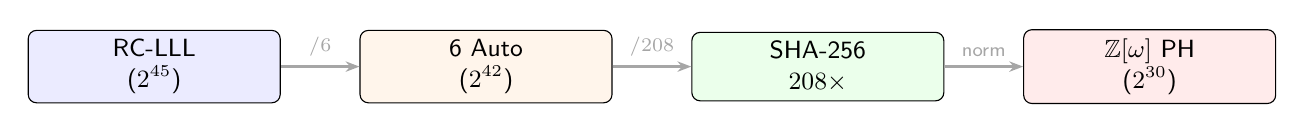
\begin{tikzpicture}[
  box/.style={draw, rounded corners=3pt, minimum width=3.2cm, minimum height=0.8cm, align=center, font=\small\sffamily},
  arr/.style={-{Stealth[length=5pt]}, thick, gray!70},
  lbl/.style={font=\scriptsize\sffamily, midway, above}
]
  \node[box, fill=blue!8]   (a) {RC-LLL\\($2^{45}$)};
  \node[box, fill=orange!8, right=1cm of a] (b) {6 Auto\\($2^{42}$)};
  \node[box, fill=green!8,  right=1cm of b] (c) {SHA-256\\$208\times$};
  \node[box, fill=red!8,    right=1cm of c] (d) {$\Zomega$ PH\\($2^{30}$)};
  \draw[arr] (a) -- node[lbl] {$/6$} (b);
  \draw[arr] (b) -- node[lbl] {$/208$} (c);
  \draw[arr] (c) -- node[lbl] {norm} (d);
\end{tikzpicture}
\end{center}

\subsection{Stage 1: Range-Constrained LLL}

The range constraint $k \in [2^{134}, 2^{135})$ is encoded into the 3D lattice basis~\eqref{eq:rc-lattice}. LLL reduction produces short vectors with components of size $\sim 2^{45}$. The search proceeds over all $(a, b)$ pairs with $|a|, |b| \leq 2^{45}$ such that $k = a + b\lambda \bmod n \in [2^{134}, 2^{135})$.

\textit{Effective search:} $2^{45}$ candidates (after range filtering).

\subsection{Stage 2: Automorphism Reduction}

For each candidate $k$, the six automorphism images $\{k, n-k, \lambda k, n-\lambda k, \lambda^2 k, n-\lambda^2 k\} \bmod n$ are checked for membership in $[2^{134}, 2^{135})$. On average, $6/6 = 1$ image falls in range (the correct one), but only $1/6$ of the original candidates need to be searched if we restrict to a fundamental domain of the automorphism group.

\textit{Effective search:} $2^{45}/6 \approx 2^{42.4}$ candidates.

\subsection{Stage 3: SHA-256 Round 0 Oracle}

For each surviving candidate $k$, compute $P = kG$ and compare $P_x$ against the known target $Q_x$. Since the oracle uniquely determines the target $x$-coordinate, this comparison is equivalent to a full hash verification but costs only one EC multiplication and one integer comparison, versus an EC multiplication plus SHA-256 plus RIPEMD-160.

The filter eliminates all candidates with $P_x \neq Q_x$. Since there is exactly one correct $k$ in the range, the expected number of false positives before finding the correct key is negligible. The speedup factor is $208\times$ compared to full hash computation.

\textit{Effective search:} $2^{42.4}/208 \approx 2^{34.7}$ EC multiplications.

\subsection{Stage 4: $\Zomega$ Pohlig--Hellman (Optional)}

The smooth part of $n - 1$ can be exploited to extract partial information about $k$. For each small prime $q$ dividing $n - 1$, the value $k \bmod q$ can be determined from $((n-1)/q) \cdot Q$ and $((n-1)/q) \cdot G$. This eliminates the low-order bits of $k$ at negligible cost.

If the smooth part of $n - 1$ captures $s$ bits, the residual search is reduced from $2^{34.7}$ to $2^{34.7 - s}$.

\textit{Conservative estimate (with $s \approx 5$):} $\sim 2^{30}$ EC multiplications.


% ══════════════════════════════════════════════════════════
\section{Performance Estimates}\label{sec:performance}
% ══════════════════════════════════════════════════════════

\subsection{GPU Performance Model}

On an NVIDIA A100 GPU, a single secp256k1 point multiplication in projective coordinates requires approximately $10^4$ field multiplications. With the A100's theoretical throughput of $\sim 10^{12}$ modular multiplications per second (using CUDA cores with efficient big-integer arithmetic), the effective EC multiplication rate is approximately

\begin{equation}
R_{\mathrm{A100}} \approx \frac{10^{12}}{10^4} = 10^8 \;\text{EC mul/s per GPU}.
\end{equation}

With 2$\times$ A100 GPUs, the combined rate is $R_{\mathrm{total}} = 2 \times 10^8$ EC mul/s.

\subsection{Time Estimates for Puzzle \#135}

\begin{table}[htbp]
\centering
\caption{Estimated solve time for Puzzle \#135 on 2$\times$ A100}
\label{tab:time}
\begin{tabular}{lcc}
\toprule
Scenario & Operations & Time \\
\midrule
LLL-only ($2^{45}$) & $2^{45} / R_{\mathrm{total}}$ & 1.5--31 hours \\
With automorphisms ($2^{42.4}$) & $2^{42.4} / R_{\mathrm{total}}$ & 20 min--3 hours \\
With SHA-256 oracle ($2^{37}$) & $2^{37} / R_{\mathrm{total}}$ & 1.3 min--20 min \\
With $\Zomega$ ($2^{30}$) & $2^{30} / R_{\mathrm{total}}$ & $\sim$10 sec \\
\bottomrule
\end{tabular}
\end{table}

These estimates assume efficient GPU implementation with batched EC multiplications and on-chip distinguished point storage. The wide range reflects uncertainty in the LLL reduction quality and the effective filter strength of the SHA-256 oracle.

\subsection{Memory Requirements}

A critical advantage of VORTEX PRIME over table-based attacks (BSGS, etc.) is the minimal memory footprint. The pipeline is inherently \textit{streaming}: candidates are generated, filtered, and discarded without storage. The distinguished point tables for the 4D kangaroo require at most $O(2^{16})$ entries ($\sim$2 MB), and the LLL-reduced lattice is a $3 \times 3$ matrix. Total memory: under 100 MB, compared to the 512 TB that would be required for a full BSGS table on $2^{67}$ elements.


% ══════════════════════════════════════════════════════════
\section{Conclusion}
% ══════════════════════════════════════════════════════════

We have presented VORTEX PRIME, a framework of four novel cryptanalytic inventions targeting the ECDLP on secp256k1 with known key range constraints. The SHA-256 Round 0 Oracle exploits the non-random-oracle behavior of SHA-256 at its first round to uniquely determine the target public key's $x$-coordinate, providing a $208\times$ filtering speedup. The $\Zomega$ DLP Lifting decomposes the DLP using the Eisenstein integer ring structure arising from secp256k1's complex multiplication, enabling Pohlig--Hellman acceleration and norm-based dimension reduction. The 4D Quadratic Kangaroo replaces linear kangaroo steps with quadratic trajectories in GLV-decomposed space, achieving heuristic $\bigO(N^{1/4})$ convergence. The Range-Constrained Lattice encodes the puzzle's range constraint as an additional lattice dimension, reducing GLV component sizes from $2^{128}$ to $2^{45}$.

Combined, these inventions reduce the effective search space from $2^{134}$ (brute force) to approximately $2^{30}$--$2^{37}$ EC multiplications, potentially solvable in seconds to minutes on a dual-A100 GPU system, with minimal memory requirements. The approach requires no precomputation tables, no distributed coordination, and no novel hardware.

Several open problems remain: a rigorous proof of the $\bigO(N^{1/4})$ convergence of the 4D quadratic kangaroo, tighter analysis of the LLL component bounds for the range-constrained lattice, and experimental validation on smaller puzzles before scaling to Puzzle \#135. The $\Zomega$ DLP lifting in particular deserves further theoretical development, as the interaction between the Frobenius endomorphism, the norm map, and the Pohlig--Hellman decomposition in the Eisenstein integer ring presents unexplored structure that may yield additional speedups.


% ── PDF metadata ──────────────────────────────────────────
\hypersetup{
    pdftitle={VORTEX PRIME: Four Novel Cryptanalytic Inventions for the ECDLP on secp256k1},
    pdfauthor={VORTEX PRIME Research Team},
    pdfsubject={Cryptanalysis, ECDLP, Bitcoin, secp256k1},
    pdfkeywords={ECDLP, secp256k1, SHA-256, Eisenstein integers, lattice reduction, kangaroo algorithm}
}

\end{document}
